% This is a template for  Masters' Theses at WPI.
% It complies (more or less) to the standards given by the Library 
% (as of February 1999)
%
% Feel free to use this file, but I give no guarantee for its compliance
% to standards (meaning I won't pay for the paper if the library rejects it :))
%
%
% The lengths (textheight, width etc.) are fine-tuned for ps1, ps2, and ps3, 
% but seem to be somewhat dependent on the machine you are using to compile, 
% the date, time, moon phase, the weather, and other quantum effects.
% You may have to change \oddsidemargin a little, but it's about 98% correct.
%
% Also, the spacing is correct (doublespacing with footnotes correctly
% singlespaced). Curiously, the font size is not specified in the
% regulations. So feel free to change it, but the majority of theses
% that I have seen is written in 12 point font.
% 
% As for the inclusion of graphics, I recommend the methods specified
% in ``latexguide.ps'' off the CS-GSO Website. You can use other
% methods including copy and paste with a photocopier, but I think
% using the graphicx package is the easiest.
%
% Have fun and good luck with the thesis.
%
%
%  Andreas Koeller (koeller@wpi.edu)
%


% The preamble
% 12 point font, and your thesis is a ``report'' to LaTeX
\documentclass[12pt]{report}

% this enables correct linespacing and graphics inclusion via 
%``\includegraphics''
\usepackage{setspace}
\usepackage{graphicx}
\usepackage{hyperref} % Chris - hyperlink all the things
\usepackage{todonotes} % Chris - nice todo notes!
\usepackage{listings} % Chris - include some code formatting stuff
\usepackage{textcomp} % Chris - fixes warnings due to gensymb below
\usepackage{gensymb} % Chris - so we can have \degrees
\usepackage{tabularx}

% leave 1.5in margin to the left and 1in margin to the other
% sides. Don't print page number in the margin (but rather above it)
\setlength{\textheight}{8.63in}
\setlength{\textwidth}{5.9in}
\setlength{\topmargin}{-0.2in}
\setlength{\oddsidemargin}{0.3in}
\setlength{\evensidemargin}{0.3in}
\setlength{\headsep}{0.0in}

% Start to write
\begin{document}

% First things first: The Titlepage
% This is the recommended format by the library
%


% Define \brk as a command for leaving a little vertical space. Makes
% the titlepage easier to read - normally, this is NOT GOOD LATEX
% STYLE!!!
%
\newcommand{\brk}{\vspace*{0.18in}}

% No page number on the title page
\thispagestyle{empty}

% Center the whole title page
\begin{center}

\brk

% Large font and bold face for the headline. Try to keep it at one or
% two lines. Headlines over two lines will mess up the spacing, and you have to
% manually finetune it. Note that the line break in the SOURCE CODE
% does not affect the line breaking in the output file. If you want
% hardcoded line breaks, you have to mark them with a double backslash (\\)

   {\large 
	\textbf{
	Constrained Motion Planning System for MRI-Guided, Needle-Based, Robotic Interventions
	}
   }


\brk
by

\brk
% insert your name here. 
Christopher Bove


% All this is constant:
\brk\brk
A Thesis DRAFT \todo{Update Draft statement.}

\brk
Submitted to the Faculty

\brk
of the 

\brk
WORCESTER POLYTECHNIC INSTITUTE
	
\brk
In partial fulfillment of the requirements for the

\brk
Degree of Master of Science

\brk
in

\brk
Robotics Engineering

\brk
by

% This is how LaTeX draws lines :) It's where your signature goes.
\brk\brk
\rule{3in}{1.2pt}

% Adjust this to your preferred month and year
\brk
May 2018

\end{center}

	
\vfill
APPROVED:

\vspace{0.25in}
\rule{3in}{0.8pt}

Professor Gregory Fischer, Major Thesis Advisor

\vspace{0.25in}
\rule{3in}{0.8pt}

Professor Zhi Jane Li, Committee Member

\vspace{0.25in}
\rule{3in}{0.8pt}

Professor William Michalson, Committee Member

% end of titlepage
\newpage

% This is the command for doublespacing when you use the setspace
% package
% Please do NOT use \baselinestretch, this will mess up everything,
% cause earthquakes, tornados and lots of questions for me...
% If you need a singlespaced paragraph (BAD STYLE!!!), use
% \singlespacing or \onehalfspacing and enclose it together with the
% paragraph in braces {\singlespacing This is my text... blah blah blah}
%
\doublespacing

% Now you can start to be creative.
% First, you need an abstract.
% Fortunately, LaTeX has thought of that, so it's very easy:
%
\begin{abstract}
\todo[inline]{Write full abstract.}
In needle-based surgical interventions, accurate alignment and insertion of the tool is paramount for providing proper treatment at the target site while minimizing healthy tissue damage. While manually-aligned interventions are well-established, robotics platforms promise to provide reduced procedure time, increased precision, and improved patient survival rates. Conducting interventions in an MRI scanner provides real-time, closed-loop feedback for the robotics platform, improving its accuracy, yet the tight environment potentially impairs motion. This project seeks to develop a surgical workflow and software system for evaluating the workspace and planning the motions of a robotics platform within the confines of an MRI scanner. 3D Slicer, a medical imaging visualization and processing platform, will provide a familiar and intuitive interface for operators to quickly plan procedures with the robotics platform. Robotics tools such as ROS and MoveIt! will be utilized to formulate the motion planning solution, analyze the workspace of the robot within the patient, and perform optimization for positioning of the robot and insertion point. For this study, a 7 DOF robot arm designed for ultrasonic ablation of brain tumors will be the targeted platform.
% This project seeks to develop a software package to generate motion plans for a 7 DOF MRI-Safe neuroablation robot for use in ultrasonic ablation of brain tumors. The solution must solve motion planning problems for two different robot configurations, and, if necessary, join the configuration states together to ensure that the robot can travel to the insertion site on the skull and insert the ultrasonic probe without colliding with the MRI machine. ROS tools such as RViz and MoveIt! will be utilized to synthesize the solution with validation using Gazebo through system simulation.
\end{abstract}

% From here on, we need Roman page numbers according to the library
% regulations. So let's assign those.

\pagenumbering{roman} % or {Roman} if you like them capitalized

% The next thing is the Preface (``Acknowledgements'').
\begin{center}
	\textbf{Acknowledgements}
\end{center}

\todo[inline]{Write acknowledgements.}

\clearpage


\tableofcontents

% THAT'S IT. REALLY. Everything else is automatic. No formatting, no headline.
% All predefined.

% Now - just as easy - the List of Figures.
% This will catch all objects enclosed in \begin{figure}\end{figure}
% statements.
\listoffigures

% There is also a list of tables, if you have any.
% This will catch all objects enclosed in \begin{table}\end{table}
% statements.
\listoftables

\clearpage

\begin{center}
	\textbf{Glossary and Notation}
\end{center}

\todo[inline]{Continue updating glossary.}
\begin{tabular}{rl}
	AIM Lab& Automation and Interventional Medicine Research Laboratory\\
	WPI& Worcester Polytechnic Institute\\
	\\
	DOF& Degrees of Freedom\\
	MOCAP& Motion Capture\\
    MRI& Magnetic Resonance Imaging\\
    Neurobot& Neuroablation Robot\\
	Pose& Position and Orientation\\
	ROS& Robot Operating System\\
	RVIZ& ROS Robot Visualizer \\
	TF& ROS Transform Library\\
	URDF& Universal Robot Description File\\
\end{tabular}

\todototoc
\listoftodos

% And we need a clear separation between preface and text, otherwise
% the numbering gets confused.

\clearpage

% And now - tataa - the text.
% This is the place to become really creative.

% From here on, we need arabic numbering again and we need to start
% from 1.

\pagenumbering{arabic}
\setcounter{page}{1}

%%%%%%%%%%%%%%%%%%%%%%%%%%%%%%%%%%%%%%%%%%%%%%%%%%%%%%%%%%%%%%%%%%%%%%%%%%%%%%%%
\chapter{Introduction}
\label{sec:intro}
\section{Clinical Problem}
Many treatments for brain cancers involve removing as much as the tumor as possible before other treatments, such as radiation or chemotherapy, are utilized to destroy the remaining tissue. Traditional procedures involve significant removal of the skull to access the tumor area, yet minimally invasive stereotactic procedures, those using 3D imaging for guidance of instruments inserted through a small hole in the skull, can reduce healthy tissue trauma, improve accuracy, and speed recovery. \cite{texasOncology}  Recent research has shown that MRI-guided ultrasonic ablation, a minimally invasive method which uses an ultrasonic probe inserted through a small hole to heat up and destroy tumor tissue, is a viable approach for treatment of brain cancers. \cite{thermalMRIAblation} 

A challenge with minimally invasive surgery is positioning the instrument and reaching the target area successfully, since the tooltip cannot be directly observed by the surgeon. Rather, it can only be visualized through MRI or ultrasound image feedback. Frames can be rigidly attached to the skull to precisely guide the instrument to the desired location \cite{texasOncology}, but significant time is required to setup these frames and verify the correct alignment. An example of this type of frame is shown in \autoref{fig:stereotactic}.

\begin{figure}[thpb]
	\centering
	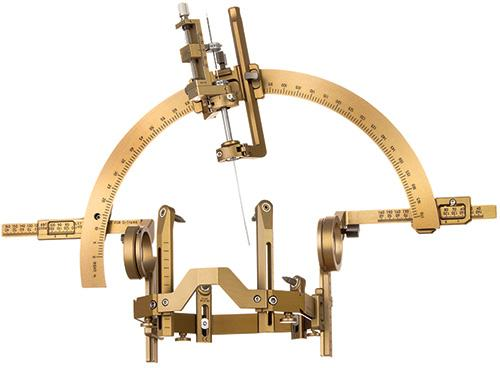
\includegraphics[width = 2.5in]{images/stereo_tactic_frame.jpg}
    \caption{A photograph of an example stereotactic frame that could be used for interventions and treatments during minimally invasive neurosurgery. \cite{stereotactic}}
    \label{fig:stereotactic}
\end{figure}

\section{Hardware Solution}
An potential alternative to manually aligning stereotactic frames is to utilize a robotic system to align the ablation tool, using closed loop feedback in both the joints (utilizing the forward kinematics of the robot) and the MRI feedback of the probe to precisely position the ablation tool at the location of the tumor. This promises significant speed and reliability improvements over manual tool alignment. Past research at WPI AIM Laboratory has produced a 5 DOF neuroablation robot which is MRI safe, lacking ferrous material, and does not distort the image significantly while operating with piezo electric motors. \cite{aimLabRobot} Kinematically, the system produces Cartesian translation from the base and orientation through a remote center of motion, emulating stereotactic frames. Newer iterations of this system provide an extra degree of freedom to rotate the ultrasonic probe for better coverage of tumors once the probe is inserted and the ability for the robot to perform the needle insertion along a separate joint. \autoref{fig:neuroRVizModel} shows the latest version of the robot in ROS RViz.

\begin{figure}[thpb]
	\centering
	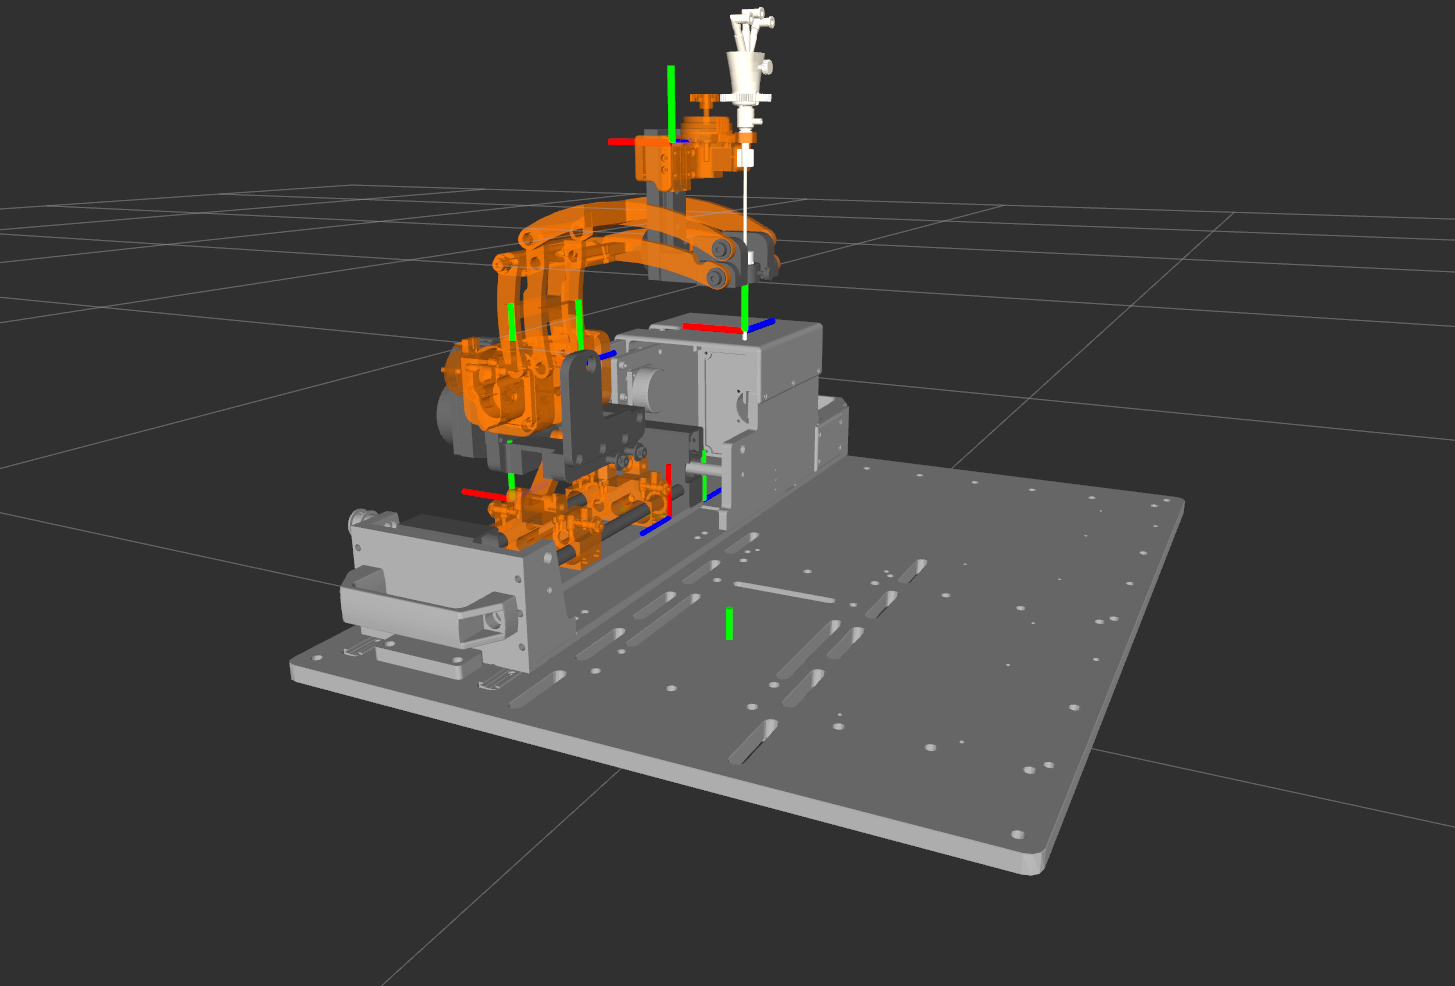
\includegraphics[width = 2.5in]{images/neuro_rviz_model.png}
    \caption{Screenshot of the neurosurgical ablation robot RViz model. Each placed frame on the robot represents a DOF. The global coordinate system is x to the left, z into the image, and y up. }
    \label{fig:neuroRVizModel}
\end{figure}

\section{Problem Statement}
When the neuroablation robot is attached to the patient table on the MRI machine, it faces several constraints that can interfere with achieving the desired needle insertion into the patient head. The robot's joint limits change based on the motions of other joints (i.e. the amount of z travel depends on the current height due to the scissor lift mechanism). With the patient rigidly placed on the table, the robot must move to achieve alignment without striking the patient's head. This is aided by removal of the ultrasonic probe and canula, as shown in \autoref{fig:neuroRVizModelNoProbe}. 

\begin{figure}[thpb]
	\centering
	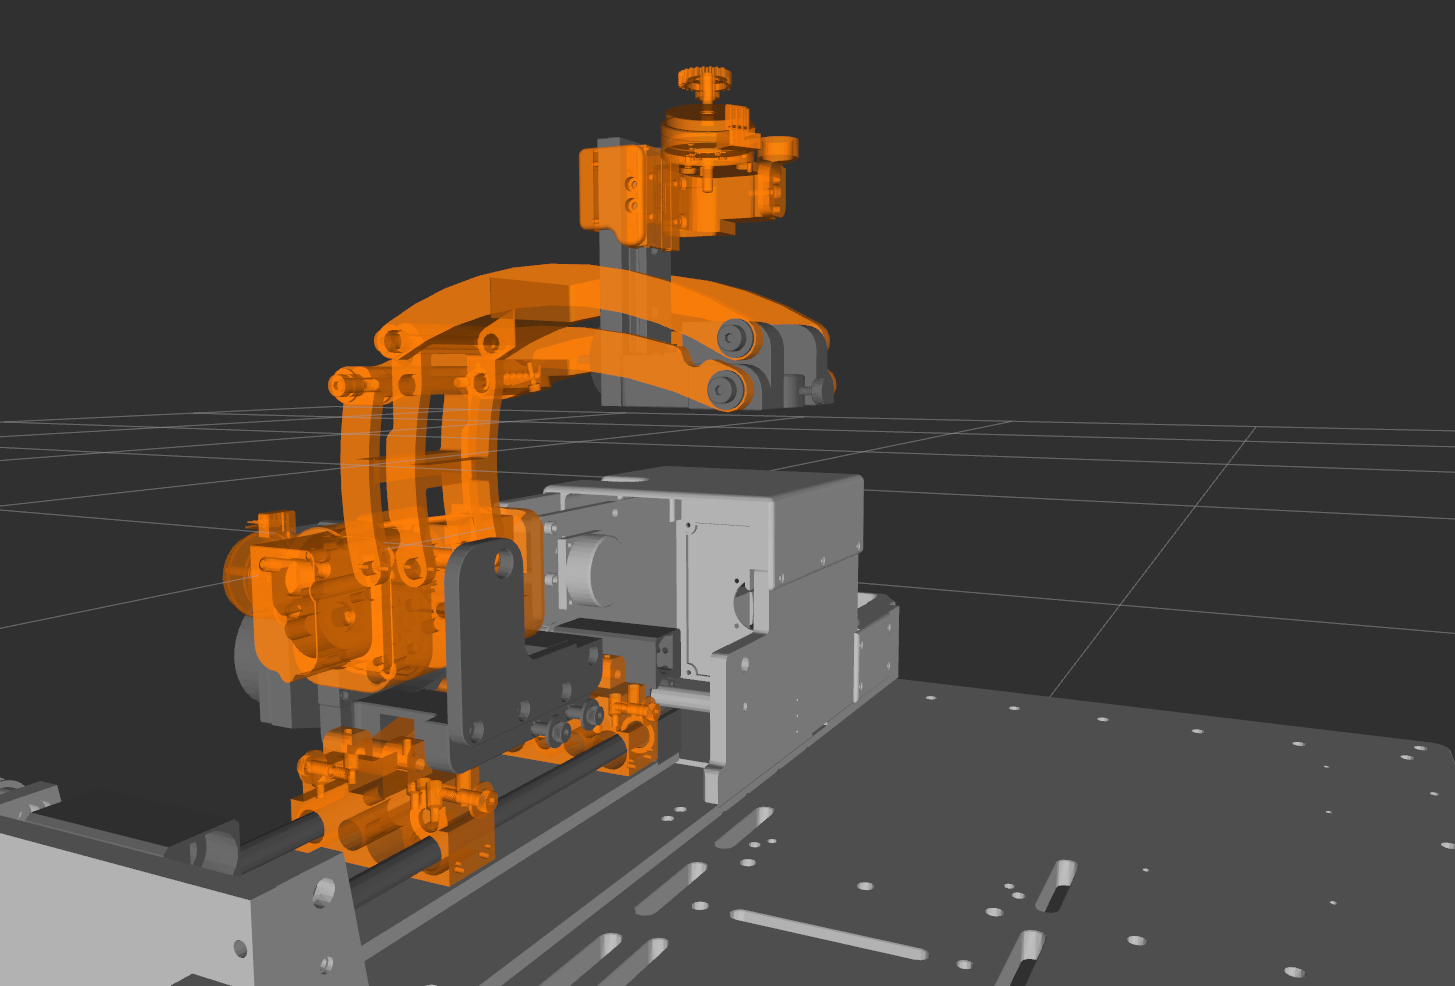
\includegraphics[width = 2.5in]{images/neuro_no_probe.png}
    \caption{Screenshot of RViz model of neurosurgical ablation robot in the configuration for positioning probe to entry point with the canula and ultrasonic probe removed. }
    \label{fig:neuroRVizModelNoProbe}
\end{figure}

Additionally, an insertion motion plan must allow the probe tip to enter through the burr hole in the skull without hitting the skull. Once the robot is in place above the burr hole, the canula is inserted into the skull and attached to the robot, and the ultrasonic ablation probe is attached to the robot and inserted into the brain by the driver DOF. This final configuration must then be able to enter the bore of the MRI machine without having the probe attachments or robot collide with the MRI machine. Therefore, a successful insertion solution must abide by the robot’s kinematic limitations, avoid collisions with the patient’s head and skull during movement to the configuration (with the canula and probe removed), have a final configuration that does not collide with the MRI bore, and reaches the target destination successfully.

Current operation of the neuroablation robot requires the coordination of two engineers to drive the robot joint-by-joint to prevent collision with the patient head and align the system to the desired insertion point. This process is time consuming and requires knowledge of the robot’s kinematic limitations and movement, increasing the difficulty for medical professionals to perform this procedure themselves. Further, the workspace of the robot given the placed burr hole in the skull is currently not visualized before the alignment is attempted. This limitation can lead to situations in which time is wasted attempting to align and reach a position that is outside the robot’s workspace, in which case the patient may need to be repositioned.

%%%%%%%%%%%%%%%%%%%%%%%%%%%%%%%%%%%%%%%%%%%%%%%%%%%%%%%%%%%%%%%%%%%%%%%%%%%%%%%%
\chapter{Background}
\section{Neuroablative Procedures}
\section{AIM Lab Neuroablation Robot Platform}

\begin{figure}[thpb]
	\centering
	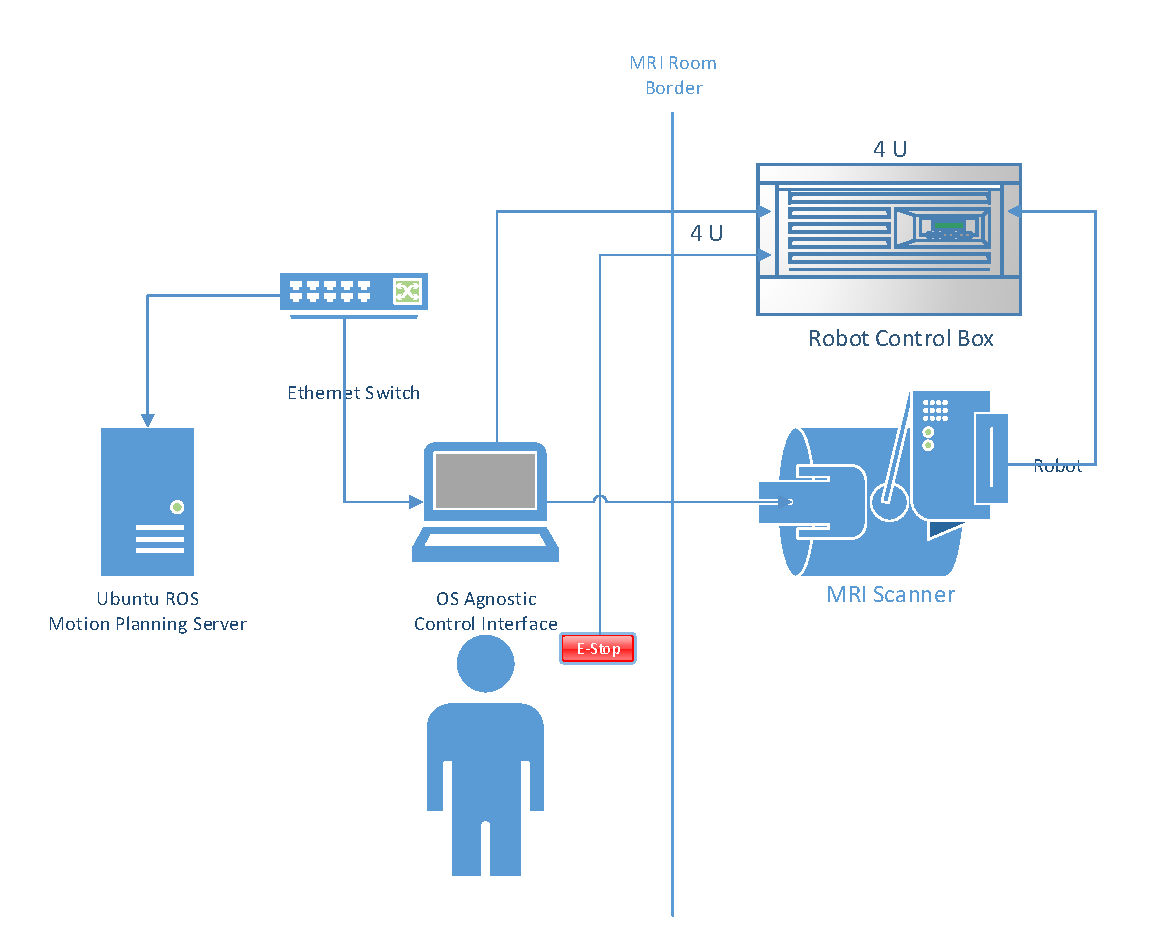
\includegraphics[width=\textwidth]{diagrams/Networking_Diagram.pdf}
    \caption{Diagram of the network interfaces between the robot, control computer, and MRI scanner. }
    \label{fig:networkDiagram}
\end{figure}

\section{Motion Planning}


\section{ROS Architecture and Tools}

\section{Medical Imaging Software: OpenIGTLink and 3D Slicer}


%%%%%%%%%%%%%%%%%%%%%%%%%%%%%%%%%%%%%%%%%%%%%%%%%%%%%%%%%%%%%%%%%%%%%%%%%%%%%%%%
\chapter{Related Work and Contributions}
\section{Motion Planning}
\label{sec:relatedWork}
Classic motion planning problems have developed several solutions that adapt to this problem well. Sampling-based approaches, such as Rapidly-exploring Random Trees (RRT) and Probabilistic Road Maps (PRM) work well for finding solutions to problems with high dimensional configuration space, as is the case in this 7 DOF system. \cite{planningAlgorithms} However, they most often fail to find optimal solutions and can be shown to most often find non-optimal solutions, prompting developments to ensure optimality such as the development of RRT*. \cite{rrtStar} Optimality is of some concern in this situation in order to reduce procedure time, but completeness and feasibility is of more importance. Given the relatively slow speed of the robot joints (after gear reduction using leadscrews), there is likely benefit to an optimal planner, yet the cost of the extra planning time to find the optimal solution could exceed the time it takes for a suboptimal path to be planned and executed.

In addition, uniform sampling methods are often very slow to find paths through narrow passages, which is a significant part of the problem for this project as the needle needs to be guided through a small opening. There are several methods for biasing task space sampling to increase configuration sampling within the narrow passages, such as using workspace features. \cite{workspaceBiasing} Such changes to the sampling may prove to be necessary in order to speed up the search time for finding viable solutions or showing that there is probably not a solution for the given problem. 

To that end, a well-developed motion planning solver, Kinodynamic Motion Planning by Interior-Exterior Cell Exploration (KPIECE), achieves a fast and robust solution for the motion planning problem by coupling, as the name suggests, dynamic aware state space searching with optimizations on searching through less-explored areas of configuration space. \cite{kpiece} KPIECE achieves noticeable computational and success rate gains compared to other algorithms such as RRT. \cite{kpiece} In addition, an implementation of KPIECE can also allow the dynamics of the robot to be considered in finding an optimal trajectory. Some of the same authors of KPIECE developed the Open Motion Planning Library (OMPL), which provides several motion planning algorithm implementations to reduce development time for robotics systems utilizing motion planning. \cite{ompl} OMPL includes an implementation of KPIECE known as LBKPIECE, which utilizes lazy collision checking (only nodes are checked for collision - edges are ignored until completing the final solution path) and bi-directional search to significantly speed searches. Utilizing OMPL, an analysis of the different motion planners was conducted, and LBKPIECE was shown to be very fast but with slightly longer than optimal path lengths. \cite{omplBenchmarks} Based on this research, LBKPIECE seems a suitable choice for this project.

\section{Neurobot Software}
\section{Contributions}
This project seeks to enhance the visualization and interaction tools available to better plan and conduct ablation procedures with the robot by generating collision-free motion plans in the interest of improving awareness of robot capabilities, reducing procedure time, and minimizing personnel involvement of manual robot alignment during ablation procedures.

%%%%%%%%%%%%%%%%%%%%%%%%%%%%%%%%%%%%%%%%%%%%%%%%%%%%%%%%%%%%%%%%%%%%%%%%%%%%%%%%
\chapter{System Design}
\section{Surgical Workflow Procedures}

\begin{figure}[thpb]
	\centering
	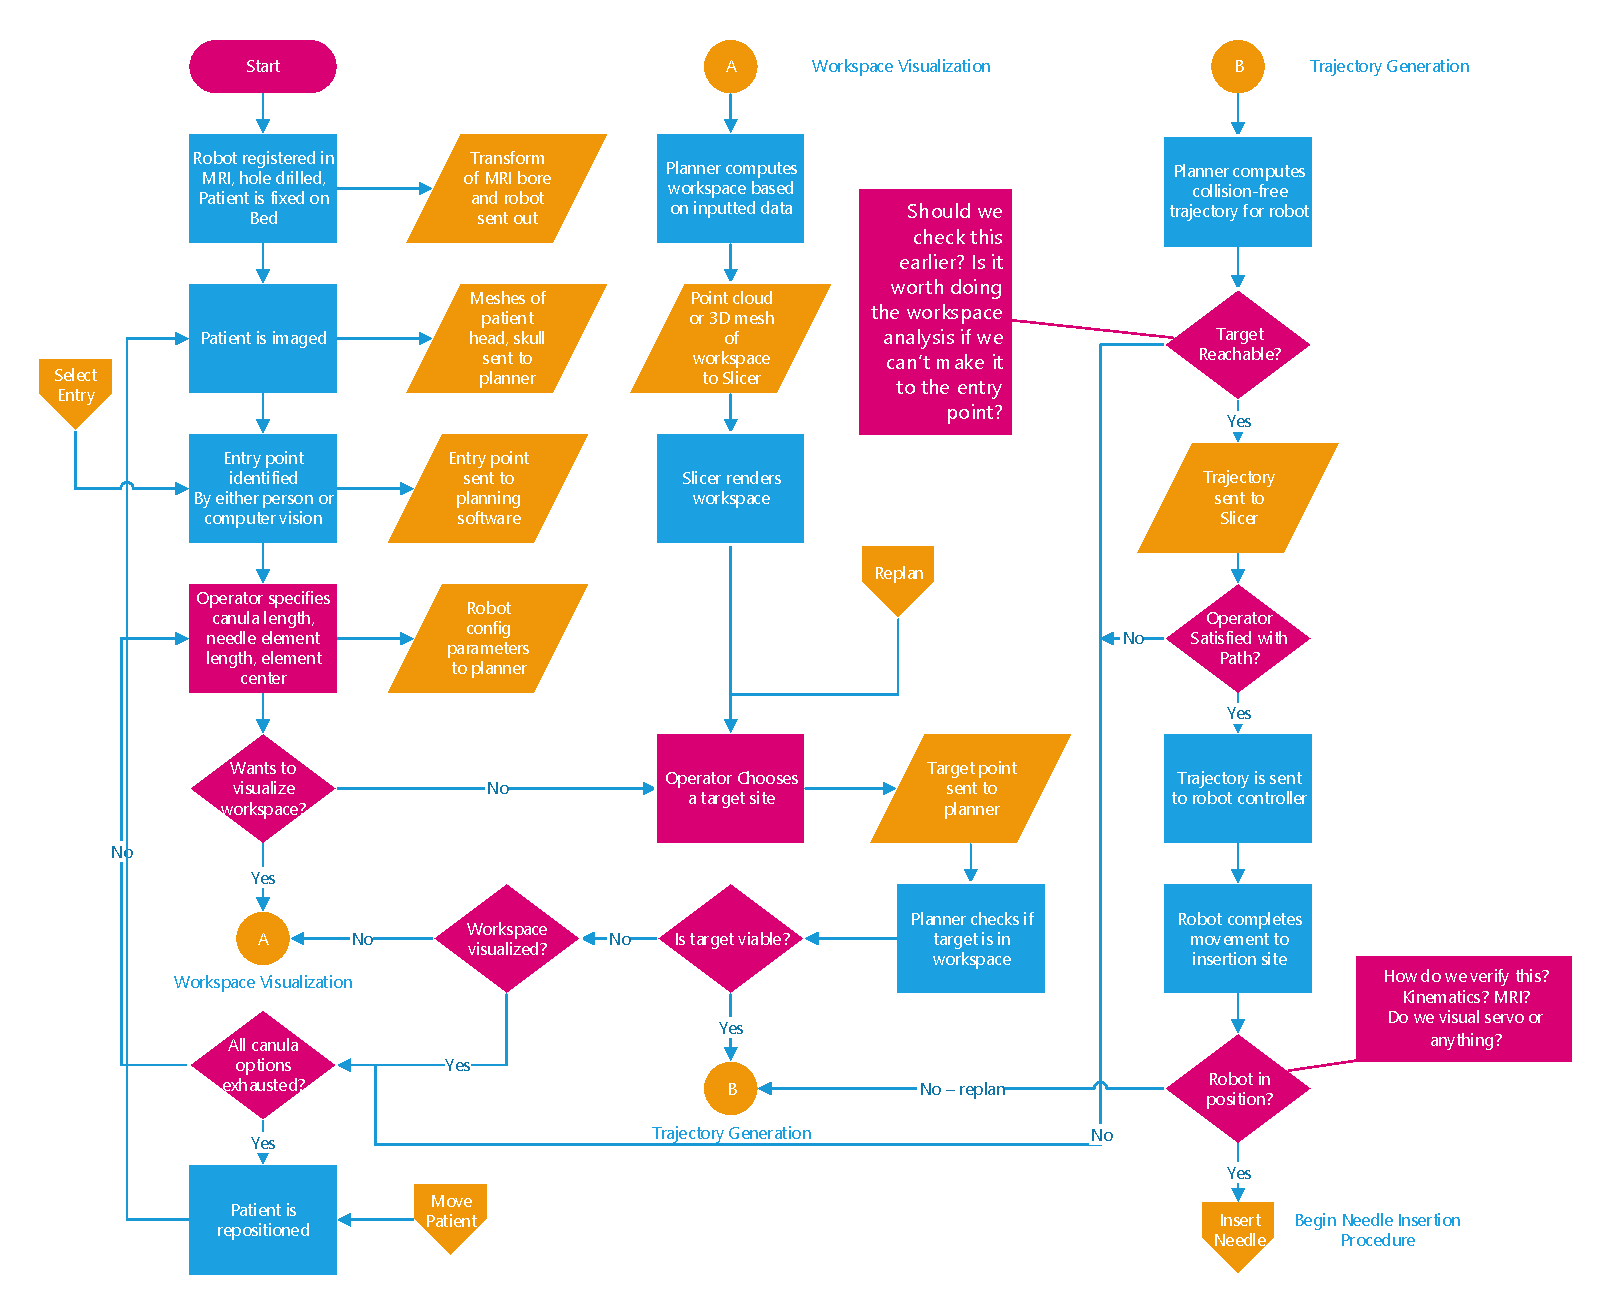
\includegraphics[page=1,width=\textwidth]{diagrams/Surgical_Workflow_-_Hole_Predrilled.pdf}
    \caption{Diagram of the surgical system workflow when the hole is drilled before the patient is placed on the MRI bed. Page 1 showing procedure setup, worskspace visualization, and trajectory generation.}
    \label{fig:surgicalWorkflowPg1}
\end{figure}

\begin{figure}[thpb]
	\centering
    \includegraphics[page=2,width=\textwidth]{diagrams/Surgical_Workflow_-_Hole_Predrilled.pdf}
    \caption{Diagram of the surgical system workflow when the hole is drilled before the patient is placed on the MRI bed. Page 2 showing needle insertion procedure and extraction.}
    \label{fig:surgicalWorkflowPg2}
\end{figure}


\section{Software Design}
\begin{figure}[thpb]
	\centering
	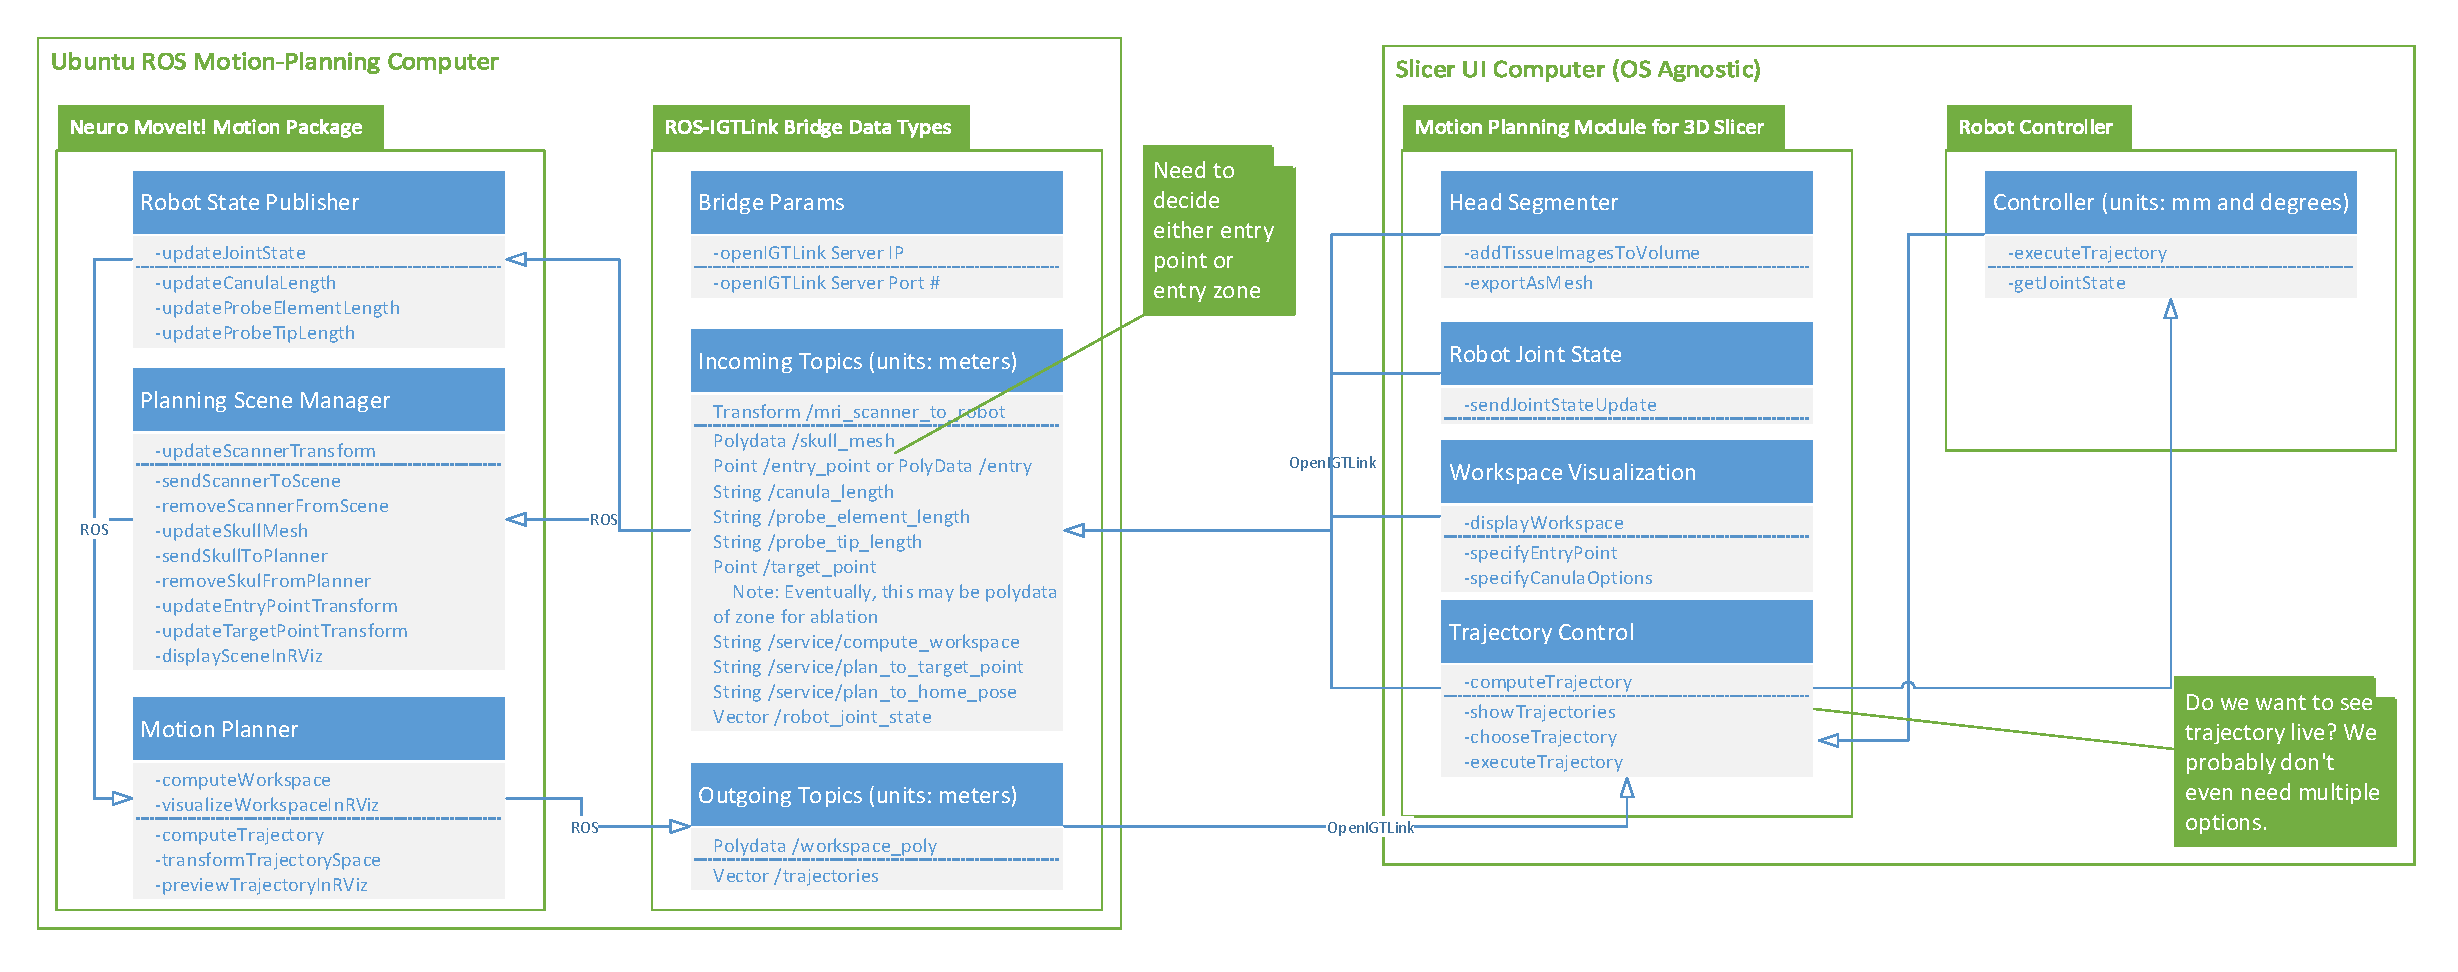
\includegraphics[width=\textwidth]{diagrams/Software_Diagrams.pdf}
    \caption{Diagram of the software architecture showing interfaces between ROS and 3D Slicer. }
    \label{fig:softwareDiagram}
\end{figure}


%%%%%%%%%%%%%%%%%%%%%%%%%%%%%%%%%%%%%%%%%%%%%%%%%%%%%%%%%%%%%%%%%%%%%%%%%%%%%%%%
\chapter{Neurobot ROS Modeling}
In order to utilize path planning and trajectory generation tools, the robot configuration will be exposed to the ROS framework, where several of these problems have already been solved by turnkey solutions, such as MoveIt!, which utilizes OMPL to provide interfaces for motion planning on robotic systems. \cite{moveIt} 
\section{Representation of Neurobot Kinematics}

\section{MoveIt! Neurobot Implementation}
Generating this particular robot model in ROS requires a bit more processing than normal. The Universal Robot Description Format (URDF) does not allow closed link loops since the joints are eventually described using TF, which expresses coordinate frames as a tree structure. This complicates the development of an accurate model and synthesis of collision models, since there are parallel linkages in the design resulting in more joints than degrees of freedom. Further, z and y motion is attained through a pair of lead screws, where the differential between the two achieves y motion and synchronized actuation produces z motion. 

The system must be modeled as a kinematic chain, so URDF mimic tags will allow the parallel linkage mechanisms to be described somewhat properly so that ROS motion planning platforms, such as MoveIt, work as desired. However, generated trajectories will have to be transformed back into the joint space of the true robot. Ideally, the IK solver utilized by MoveIt will suffice, though a custom solver implemented with IKFast may be necessary to cope with these differences from the URDF robot to the actual mechanism and speed the execution to be acceptable. \cite{ikFastMoveIt} By default, MoveIt! utilizes the Orocos Kinematics and Dynamics Library (KDL), which can describe and develop IK solutions for a number of different kinematic systems. \cite{orocosKDL} KDL also provides collision checking with the robot itself and the surrounding environment. Additionally, the RVIZ plugin will be utilized for allowing quick control and interaction with the robot model to visualize reachable areas and for considering manipulability in certain robot configurations.

%\subsection{Neurobot Model Control}
\section{Environmental Modeling}
The MRI bore and human head models will be loaded as STL files into the MoveIt! framework so that they can be utilized as a collision scene for motion planning purposes. The final result of such imports is shown in \autoref{fig:mriBore}

\begin{figure}[thpb]
	\centering
	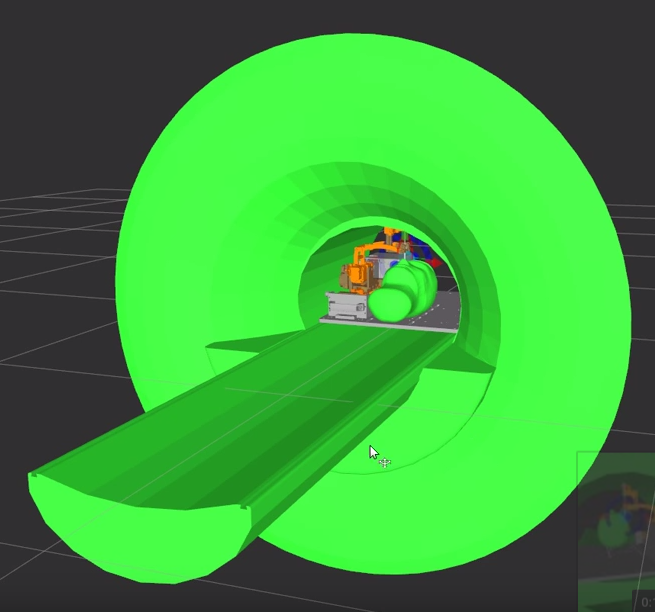
\includegraphics[width = 3in]{images/mri_bore_and_head.png}
    \caption{An image from RVIZ showing the MRI Bore model and human head model loaded with the robot utilizing the MoveIt! API from within a C++ node.}
    \label{fig:mriBore}
\end{figure}

\section{System Interaction and Visualization}

%%%%%%%%%%%%%%%%%%%%%%%%%%%%%%%%%%%%%%%%%%%%%%%%%%%%%%%%%%%%%%%%%%%%%%%%%%%%%%%%
\chapter{Workspace Examination}
\section{Basic Workspace Visualization}
Given an entry point in the skull, the workspace of the robot needs to be visualized in order for operators to verify that the chosen patient and robot positions will allow the targeted site to be reached adequately. An analytical solution would be most elegant, though a discretized solution would also produce the desired outcome. As an initial implementation, the entry point will be given, and the proposed software system will calculate the reachable workspace of the robot at that entry point. This will require the borehole diameter and skull thickness, which will be provided by an STL model of a typical skull. \autoref{fig:workspace} shows a sample of the desired visualization.

\begin{figure}[thpb]
	\centering
	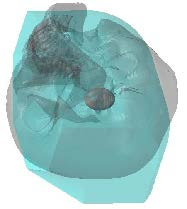
\includegraphics[width = 1.25in, angle=180]{images/neuro_workspace.jpg}
    \caption{Example 3D rendering of robot workspace without consideration of entry point location with ellipsoid of target for deep brain stimulation. \cite{aimLabRobot} This project will implement the rendering in RViz.}
    \label{fig:workspace}
\end{figure}

The approach will be to sample from configuration space, passing joint values through a self-collision aware IK solver (either from MoveIt or the Java implemented controller for the robot software), to generate a point cloud of reachable needle tip positions. This cloud will then be wrapped in a mesh and exported through OpenIGTLink so that Slicer3D, a medical imaging research tool, can display the proper workspace within the skull in the context of the rest of the robot control system. \autoref{fig:workspaceAct} shows the achieved workspace visualization.

\begin{figure}[thpb]
	\centering
	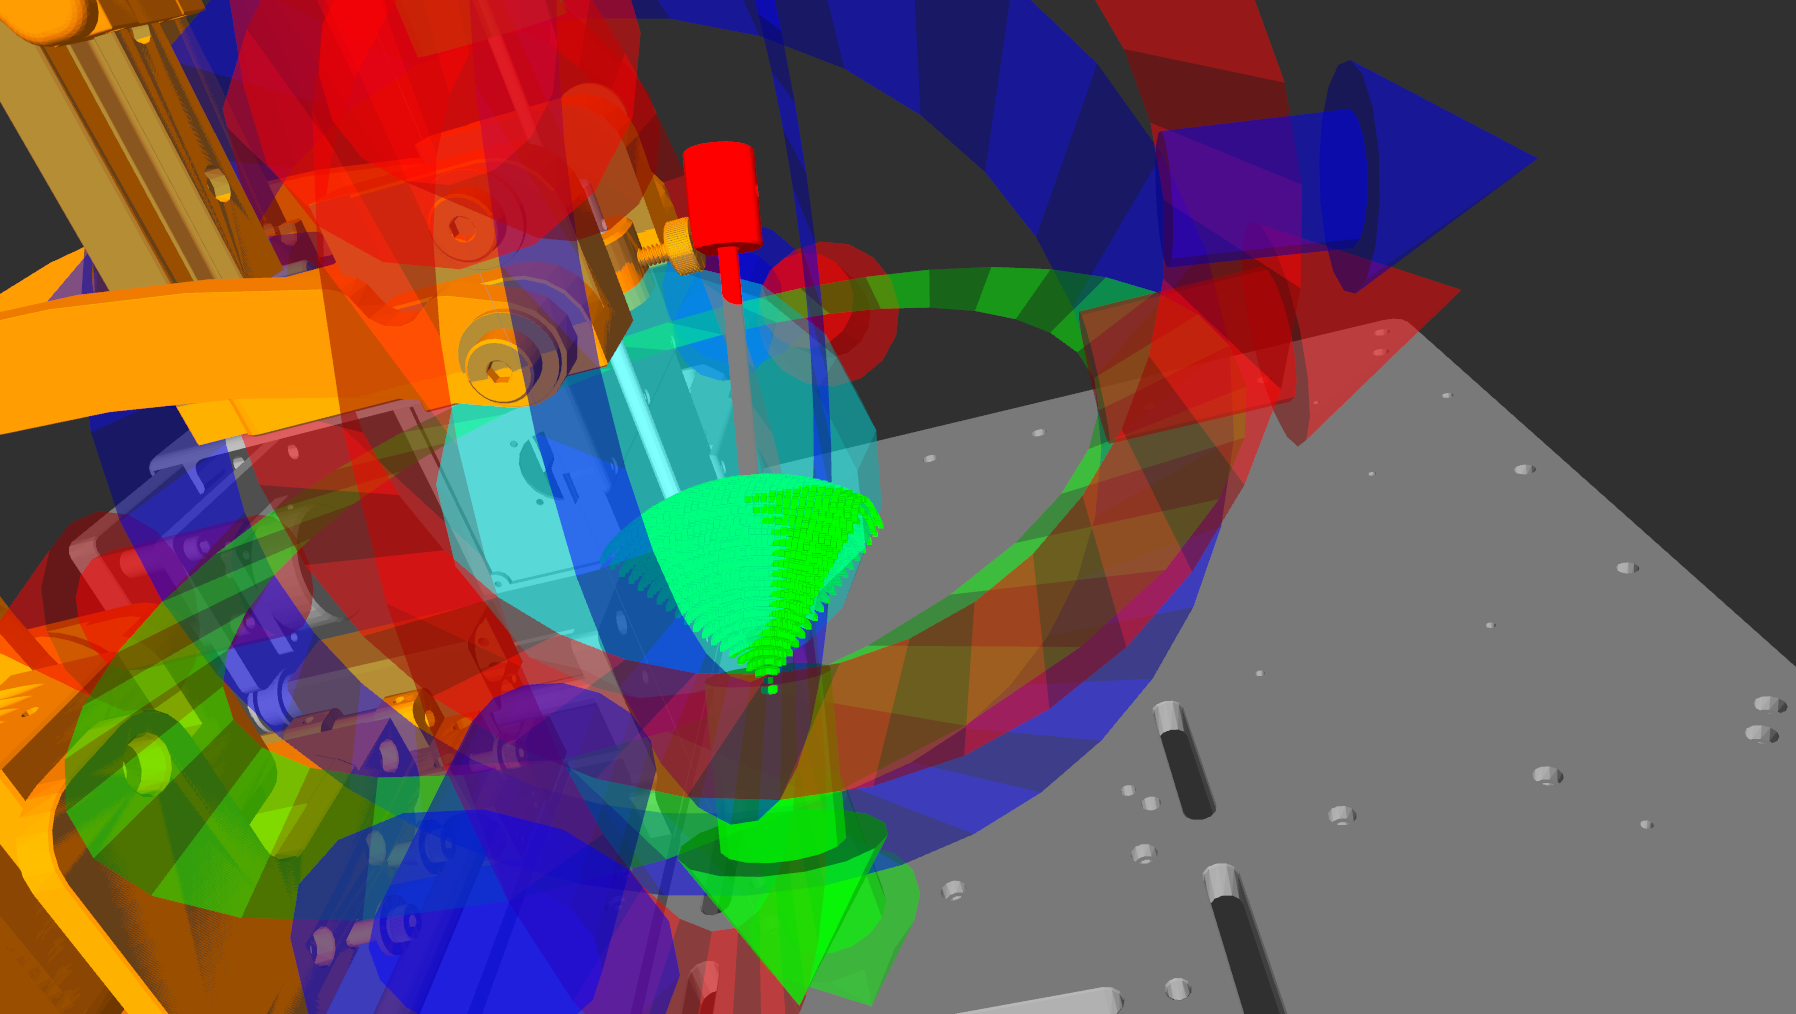
\includegraphics[width = 2.5in]{images/workspace_v1.png}
    \caption{RViz screenshot of the generated workspace (green) given the canula position (red) within the MoveIt interface.}
    \label{fig:workspaceAct}
\end{figure}

\section{Collision-Aware Workspace Examination}

\section{Manipulability Analysis}


%%%%%%%%%%%%%%%%%%%%%%%%%%%%%%%%%%%%%%%%%%%%%%%%%%%%%%%%%%%%%%%%%%%%%%%%%%%%%%%%
\chapter{Motion Planning}
\section{Generating Trajectories with MoveIt!}
In effect, two separate motion planning problems need to be solved for the two different configurations of the robot during the procedure outlined in \autoref{sec:intro}. To reiterate, during the first step, the robot is outside of the MRI bore and does not have the needle driver installed. This allows the robot to move without the constraints of the needle driver hitting the patient head and the rest of the robot striking the MRI bore. However, once the robot has moved to the entry point, the needle driver is added and inserted to the required depth, and the patient bed is slid into the MRI tube.

To simplify the problem, a solution can attempt to be found for aligning the robot without the probe, and then collision between the probe and MRI tube can be checked once the probe was inserted. If there was no collision, then the solution is valid and the trajectory can be executed. However, if the probe will collide with the MRI tube, then another planning session must begin considering the second robot configuration, where the c-space around the insertion point must be searched for a collision free state. For each one that is found, meaning that the probe can be inserted to depth and be collision free, a path to that state without the probe (first configuration) needs to be found as well to ensure it is reachable from the initial robot state. In this way, the problem of having two configurations to plan can be sufficiently handled.

As discussed in \autoref{sec:relatedWork}, LBKPIECE is supported by MoveIt! and produces faster trajectories that other motion planning algorithms. Unfortunately, the MoveIt! wrapper does not expose the ability to manipulate or change cost functions. Thus the default cost function was utilized, which optimized the path distance. Below are the available configuration options and the values chosen for the experiments. \autoref{fig:traj} shows an example trajectory being executed within RVIZ given this configuration for the needle planning group.

\begin{enumerate}
\item border fraction: 0.9
\item failed expansion score factor: 0.5
\item goal bias: 0.05
\item min valid path fraction: 0.5
\item border fraction: 0.9
\item min valid path fraction: 0.5
\item range: 0.0
\item type: geometric::LBKPIECE
\end{enumerate}

\begin{figure}[thpb]
	\centering
	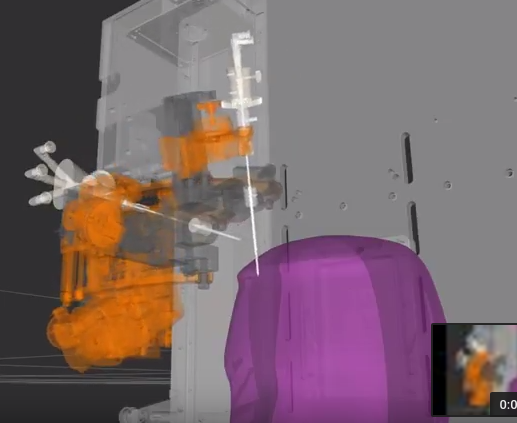
\includegraphics[width = 2.5in]{images/traj.png}
    \caption{RViz screenshot of a trajectory being completed, though without proper collision checking of the head model inserted into the world.}
    \label{fig:traj}
\end{figure}
\section{Transforming Joint Space Trajectories}

\section{Creating Collision-Free Trajectories}

%%%%%%%%%%%%%%%%%%%%%%%%%%%%%%%%%%%%%%%%%%%%%%%%%%%%%%%%%%%%%%%%%%%%%%%%%%%%%%%%
\chapter{System Implementation}
\section{Bridging with OpenIGTLink}
\section{Receiving Robot State}
\section{Sending Joint Trajectories}
\section{Real-time Execution}

%%%%%%%%%%%%%%%%%%%%%%%%%%%%%%%%%%%%%%%%%%%%%%%%%%%%%%%%%%%%%%%%%%%%%%%%%%%%%%%%
\chapter{MRI Segmentation}

%%%%%%%%%%%%%%%%%%%%%%%%%%%%%%%%%%%%%%%%%%%%%%%%%%%%%%%%%%%%%%%%%%%%%%%%%%%%%%%%
\chapter{Optimization of Patient Head Positioning}
\section{Description of Optimization Problem}
The patient head position and orientation could be optimized to provide the robot with greatest manipulability around the target area. This would involve consideration of the target area, typical burr hole locations on the skull, comfortable range of motion of the patient’s head, and the flexibility of robot mounting locations. Though a challenging problem to solve, this could remove some of the uncertainty and replanning that occurs during procedures due to a patient position that prevents the robot from reaching the target site.
\section{Implementation of Optimization Solution}

%%%%%%%%%%%%%%%%%%%%%%%%%%%%%%%%%%%%%%%%%%%%%%%%%%%%%%%%%%%%%%%%%%%%%%%%%%%%%%%%
\chapter{Experiments}
\section{Motion Planning Benchmarking}
\todo[inline]{Refreshed and rethink benchmarking.}
Several experiments were conducted in order to gain a better understanding of the execution time of the IK solver and the motion planning implementation. Tests were configured by determining a viable end effector needle pose by uniform random sampling from the configuration space of the robot and using the forward kinematics to compute the end effector position. This position was then fed back into the IK solver and the time it took the IK solver to compute the solution was measured. There were several variations of this test, but collision checking with the environment was not implemented.

In the first experiment, the parameters of the IK solver, namely the number of allowed solver attempts and the allowed search time, were set at default values of 5 attempts and 0.01 seconds. \autoref{fig:ikTimeFixed} shows the execution time plotted over 200 iterations of the solver. Interestingly, the solving time is somewhat dependent on the order of the queries: the initial query takes the longest and the number of long queries decreases over time. This seems to indicate a weak caching optimization to speed up processing.

\begin{figure}[thpb]
	\centering
	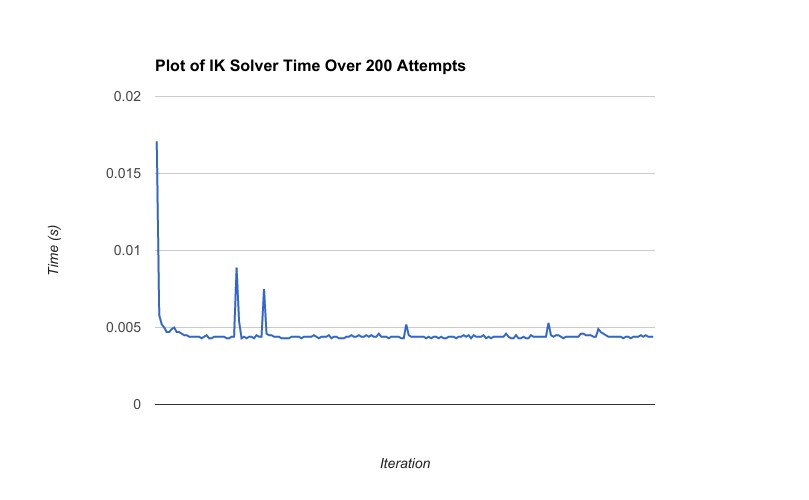
\includegraphics[width = 3.5in]{graphs/ik_solver_fixed_stats.png}
    \caption{Plot of inverse kinematics solver execution time to find viable joint configuration in collision free environment given a random reachable target over 200 consecutive trials. Average 0.004546s. 5 allowed attempts with 0.01s to find configuration.}
    \label{fig:ikTimeFixed}
\end{figure}

In the next experiment, the number of attempts was fixed at 1 and the time allowed for finding solutions was varied from 0.00001s to 0.00991s. \autoref{fig:ikexeTime} shows the results of the experiment. While a slight minimum appeared around 0.003s, there was not a strong trend, other than in longer search times, the execution time generally increased. \autoref{fig:ikHist} shows the same data but as a histogram plot.

\begin{figure}[thpb]
	\centering
	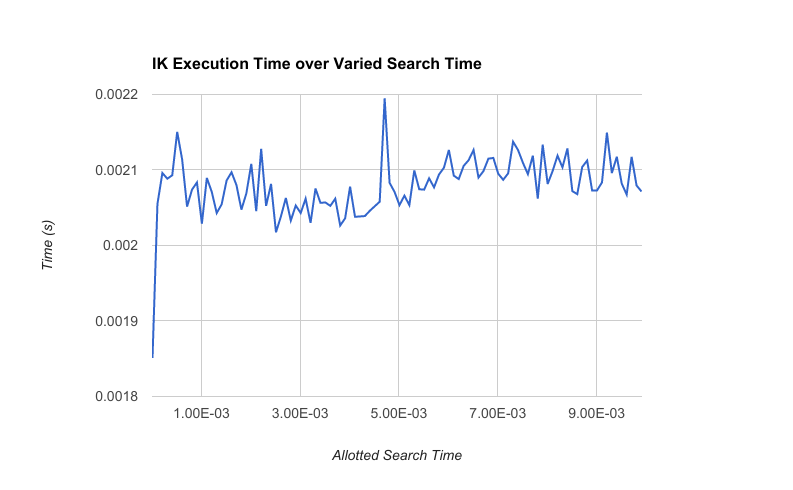
\includegraphics[width = 3.5in]{graphs/ik_exec_time_over_allowed.png}
    \caption{Plot of inverse kinematics solver execution time over allotted search time to find viable joint configuration in collision free environment given a random reachable target. 200 trials.}
    \label{fig:ikexeTime}
\end{figure}

\begin{figure}[thpb]
	\centering
	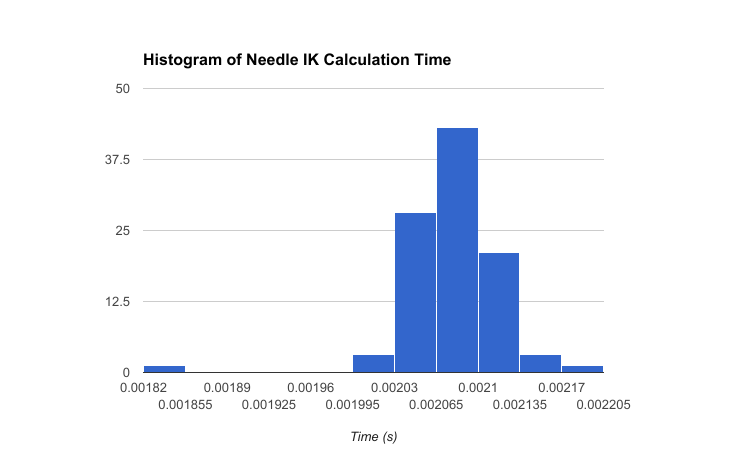
\includegraphics[width = 3.5in]{graphs/ik_hist_1_attempt.png}
    \caption{Histogram plot of inverse kinematics solver execution time to find viable joint configuration in collision free environment given a random reachable target. 200 trials. Average 0.00207957s}
    \label{fig:ikHist}
\end{figure}

In the final experiment with the IK solver, the number of attempts allotted to the solver was varied from 1 to 19, with 200 tests being conducted for each timing point. \autoref{fig:ikNumAttempts} shows the results of the test. Perhaps somewhat unsurprisingly, with only 1 attempt at solving the IK, the average execution time was highest since failure to find a solution would maximize the timeout allowed on the search without being able to spawn another. Beyond 2 allowed attempts, there is no strong trend, indicating that the choice does not matter.

\begin{figure}[thpb]
	\centering
	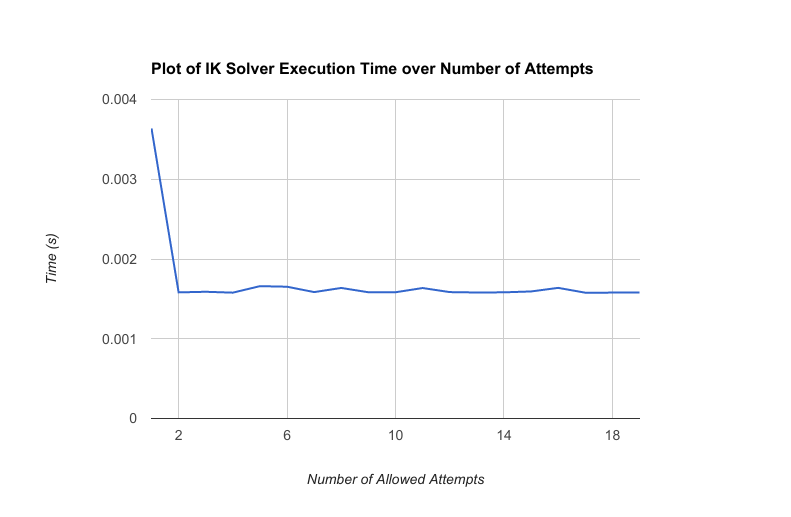
\includegraphics[width = 3.5in]{graphs/ik_sover_over_time.png}
    \caption{Plot of inverse kinematics solver execution time over number of allowed attempts to find viable joint configuration in collision free environment given a random reachable target. 200 trials averaged for each number of allowed attempts. Average 0.001707s}
    \label{fig:ikNumAttempts}
\end{figure}

The motion planner was examined in the next set of experiments. Similarly to the tests for the IK solver, the same random valid configuration generation was used to set a desired pose to the needle planning group. \autoref{fig:plannerHist} indicates that most planning sessions lasted from 0.1s to 
0.225s with a tail towards longer execution times. However, no plans took longer than 0.5 second to generate, even given a limit of 5 seconds. This is beneficial to see during the collision free tests, but likely increases to several dozen seconds once large meshes are added to the environment and considered.

\begin{figure}[thpb]
	\centering
	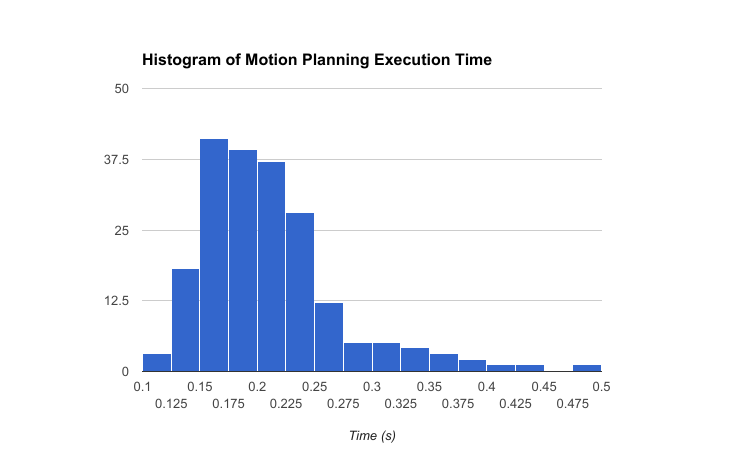
\includegraphics[width = 3.5in]{graphs/planner_hist.png}
    \caption{Histogram plot of motion planner execution time to find path in collision free environment between 2 random configurations. 200 trials. Average 0.209805s}
    \label{fig:plannerHist}
\end{figure}

The path smoothing operation was also examined in some detail. \autoref{fig:pathHist} shows the execution time of the path smoothing algorithm, which indicates a relatively narrow distribution with a tail end towards longer execution times, similar to the distribution of planner times. This is expected as more complex trajectories take longer to generate and will consume more time to process. In general, the path smoothing is a very small part of the total path planning operation.

\begin{figure}[thpb]
	\centering
	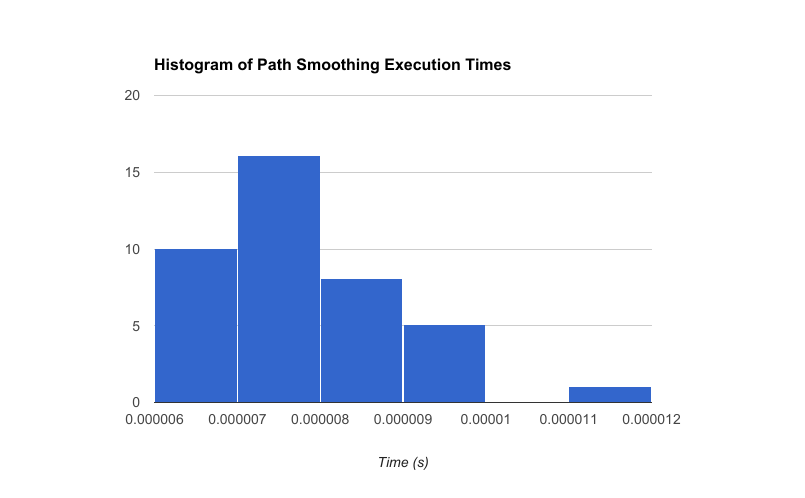
\includegraphics[width = 3.5in]{graphs/smoother_hist.png}
    \caption{Histogram plot of motion planner path smoothing execution time. 40 trials. Average 0.0000073s}
    \label{fig:pathHist}
\end{figure}
\subsection{Collision-Free Planning}
Links to video demonstration of the system performing the above actions can be found in \autoref{sec:appendixVideos}.
\subsection{Environment Collision-Aware Planning}

\section{Patient Head Optimization Results}

\section{System Validation}


%%%%%%%%%%%%%%%%%%%%%%%%%%%%%%%%%%%%%%%%%%%%%%%%%%%%%%%%%%%%%%%%%%%%%%%%%%%%%%%%
\chapter{Conclusions}
\todo[inline]{Revise Conclusions.}
This project demonstrated implementation of a LBKPIECE algorithm utilizing the OMPL through the MoveIt! API and manipulation of such an implementation for computing workspace reachability and generating trajectories of a 7DOF robot to move an end effector to an entry point. While the proposed project direction was not flawed, time for learning the MoveIt! API was underestimated. It took longer than expected to import the models properly into the planning scene, and a failure to understand the workflow of the API earlier in development did not allow the published collision scene to be reapplied to the local robot environment created in the developed plugin. The issue can be fixed with additional understanding of the API and a rewriting of the implemented node.

Results and testing show that the system will, when completed, perform the desired tasks sufficiently quickly to be useful on the actual robot hardware. Trajectory generation to a valid pose consumed an average of 0.21 seconds with no collision objects, and as the motion of the robot to an entry point on the skull will generally be collision free, this approach promises to be significantly faster than manually planning and executing trajectories by driving the robot joint by joint in the operating room (several minutes). 

Moving forward, MoveIt! appears to be a reasonable platform for developing a `turn-key' motion planning system, yet it does mask several more advanced features of OMPL from the user. For instance, cost functions cannot be modified; they are locked to OMPL defaults by the MoveIt! interface. \cite{moveitIssue} In order to adjust cost functionality currently, OMPL needs to be utilized directly without the MoveIt! wrapper. This would significantly increase development time, but could prove advantageous in other ways. ROS URDF file format cannot model parallel robots, yet KDL does allow for solving parallel kinematic chains. \cite{kdl} So there could be benefit to directly interfacing with KDL and OMPL, yet the benefits of the MoveIt! framework tend to offset its drawbacks for typical use cases.

%%%%%%%%%%%%%%%%%%%%%%%%%%%%%%%%%%%%%%%%%%%%%%%%%%%%%%%%%%%%%%%%%%%%%%%%%%%%%%%%
\chapter{Future Work}
\todo[inline]{Update future work.}
Future work will focus on properly controlling the collision environment to ensure collision-checking works properly within the developed node. Future workspace checking will then be able to use a model of the skull and burr hole for very accurately determining the workspace within the skull itself. Trajectories will be transformed back into the joint space of the actual robot hardware and passed over the software interface currently utilized in AIM Lab. Finally, the patient head pose and burr hole location can be optimized to ensure maximum reachability around the tumor location by porting the robot model into OpenRave and utilizing existing optimality planners for determining where to locate the base of industrial robot manipulators. \cite{workspaceChecker} With the robot model properly represented in OpenRave, a functioning IKFast plugin could be created as well to enable analytical solving of the IK of the robot.


\appendix
\chapter{Video Demonstrations}
\label{sec:appendixVideos}
Videos of the system in operation are listed below:
\begin{enumerate}
\item Robot and joint movements visualized in RViz \url{https://youtu.be/A8vxQcD-D1M}
\item MoveIt! Planning Scene with MRI Bore and head \url{https://youtu.be/uBkmzkpJ0bE}
\item Collision-aware IK in MoveIt! Scene \url{https://youtu.be/aWqPCrOiD8k}
\item Workspace checking demonstration \url{https://youtu.be/w9iJODJL3ho}
\item Trajectory planning demonstration with canula \url{https://youtu.be/qjk9I6ZQJBc}
\item Trajectory movement with needle tip planning group \url{https://youtu.be/b-VsMk519GQ}
\end{enumerate}

% you can save some space by having the bibliography singlespaced, if you want
\singlespacing

%
% You should become familiar with the BibTeX program, which
% uses a *.bib-file to collect all citations that you have. It's a lot
% prettier than typing all the citations right into the document. The 
% reference to citations also works well that way, but the exact 
% explanation of that will be on the CS-GSO homepage, whenever I'll ever 
% have time for that.
%
%
% If you use BibTeX, the bibliography is very easy. You refer to
% citations in the text with \cite{tag}, where tag is the tag that you
% defined in the bib-file.
% Then, you run bibtex once in a while during compilation, and the
% rest is done in two lines:

\begin{thebibliography}{99}

\bibitem{texasOncology} Texas Oncology. ``Brain Tumor Surgery.'' Accessed 2017. Online at \url{http://www.texasoncology.com/types-of-cancer/brain-cancer/surgery-for-brain-tumors}

\bibitem{thermalMRIAblation} Coluccia, Daniel, et al. ``First noninvasive thermal ablation of a brain tumor with MR-guided focusedultrasound.'' Journal of therapeutic ultrasound 2.1 (2014): 17. \href{https://jtultrasound.biomedcentral.com/articles/10.1186/2050-5736-2-17}{Link}

\bibitem{stereotactic} Elekta. ``Lesell Stereotactic System.'' Online at \href{https://www.elekta.com/neurosurgery/leksell-stereotactic-system.html}{Link}

\bibitem{aimLabRobot} Li G, Su H, Cole GA, Shang W, Harrington K, Camilo A, Pilitsis JG, Fischer GS, ``Robotic System for MRI-Guided Stereotactic Neurosurgery,'' IEEE Transactions on Biomedical Engineering, Vol 64, No 4, pp 1088-1088, April 2015. \href{http://aimlab.wpi.edu/includes/publications/2014_TBME_Li_Fischer_RoboticSystemforMRIGuidedStereotacticNeurosurgery.pdf}{Link}
% desire: include uncertainty rrt thing
\bibitem{planningAlgorithms} LaValle, Steven M. ``Planning algorithms.'' Cambridge university press, 2006. \href{http://citeseerx.ist.psu.edu/viewdoc/download?doi=10.1.1.225.1874&rep=rep1&type=pdf}{Link}
\bibitem{rrtStar} Karaman, Sertac, and Emilio Frazzoli. ``Sampling-based algorithms for optimal motion planning.'' The international journal of robotics research 30.7 (2011): 846-894. \href{http://citeseerx.ist.psu.edu/viewdoc/download?doi=10.1.1.419.5503&rep=rep1&type=pdf}{Link}
\bibitem{workspaceBiasing} Zucker, Matt, James Kuffner, and J. Andrew Bagnell. ``Adaptive workspace biasing for sampling-based planners.'' Robotics and Automation, 2008. ICRA 2008. IEEE International Conference on. IEEE, 2008. \href{http://www.ri.cmu.edu/pub_files/pub4/zucker_matthew_2008_1/zucker_matthew_2008_1.pdf}{Link}

\bibitem{kpiece} Sucan, Ioan A., and Lydia E. Kavraki. ``Kinodynamic motion planning by interior-exterior cell exploration.'' Algorithmic Foundation of Robotics VIII. Springer Berlin Heidelberg, 2009. 449-464. \href{http://www.wafr.org/wafr2008/papers/wafr08-sucan.pdf}{Link}

\bibitem{ompl} Sucan, Ioan A., Mark Moll, and Lydia E. Kavraki. ``The open motion planning library.'' IEEE Robotics \& Automation Magazine 19.4 (2012): 72-82. \href{http://ieeexplore.ieee.org/abstract/document/6377468/}{Link}

\bibitem{omplBenchmarks} Moll, Mark, Ioan A. Sucan, and Lydia E. Kavraki. ``An extensible benchmarking infrastructure for motion planning algorithms.'' arXiv preprint arXiv:1412.6673 (2014). \href{https://arxiv.org/pdf/1412.6673.pdf}{Link}

\bibitem{orocosKDL} Bruyninckx, Herman. ``OROCOS: design and implementation of a robot control software framework.'' Proceedings of IEEE International Conference on Robotics and Automation. 2002. \href{http://citeseerx.ist.psu.edu/viewdoc/download?doi=10.1.1.415.9503&rep=rep1&type=pdf}{Link}

\bibitem{moveIt} Sucan, I. A., and Chitta, S. (2013). ``Moveit!.'' Online at \url{http://moveit.ros.org.}
\bibitem{ikFastMoveIt} Sucan, I. A., and Chitta, S. (2016). ``Moveit! IKFast Plugin Tutorial.'' Online at \url{http://docs.ros.org/kinetic/api/moveit_tutorials/html/doc/ikfast_tutorial.html}

\bibitem{moveitIssue} Sucan, I. A., and Chitta, S. (2013). ``ros-planning moveit issue 118'' Online at \url{https://github.com/ros-planning/moveit/issues/118}

\bibitem{kdl} Orocos Kinematics and Dynamics. ``KDL Wiki.'' Accessed April 2017. Online at \url{http://www.orocos.org/kdl}

\bibitem{workspaceChecker} ROS.org ``reuleaux package documentation.'' Accessed April 2017. Online at \url{http://wiki.ros.org/reuleaux}

\end{thebibliography}

% \bibliographystyle{alpha}
% \bibliography{foo}

% which assumes a file foo.bib in your working directory.
% The word ``Bibliography'' will appear in your document as soon as
% you used ``bibtex'' on the command line.
%
% For reference on this, refer to the CS-GSO homepage.

%============================
%That's all, folks. Have fun.
%
%                     Andreas
%============================


\end{document}


% % Since this is a ``report'', the topmost level of hierarchy is
% % ``Chapter'', not section as you may be used to. Chapters are
% % enumerated starting from 1, so Sections are 1.1, Subsections are
% % 1.1.1, subsubsections don't get numbers. (You can change that, if
% % you want them to be called 1.1.1.1)
% %
% \chapter{First Chapter.}
% This should ideally contain some text.
% \section{First Section.}
% More Text.
% \subsection[Alternative title for the Table of Contents]{First Subsection.}
% Even more text, maybe a formula:
% \begin{equation}
% \sum_{i=1}^{n}i=\frac{n(n+1)}{2} % much easier than Microsoft Equation
%                                  % Editor :)
% \end{equation}
% \subsubsection{First Sub-subsection.}
% This is really deep down in the hierarchy. Maybe you shouldn't even
% use sub\-subsections. It goes further down (paragraphs), but I don't
% think you'll need that\footnote{By the way: notice that, although we
% have doublespacing here, the footnotes are singlespaced. This is
% intended and good. If you want to change that, try, but this is really
% how it should be.}.

% \section{Other thoughts.}
% Okay, what else?
% Let me quickly put a figure here, maybe a piece of pseudo code.
% That way, you can see how this is done. It's a little painful, but
% looks really cool. We will call it Figure~\ref{fig:source_algo1}. The
% numbering is automatic---don't worry about it.

% %First, we want to make our life easier and define a ``TAB'' command.
% \newcommand{\T}{\hspace*{5mm}}

% % Start a figure
% \begin{figure}[htb]
% % We would like to have the whole thing in the center of the page
% \begin{center}
% % We want a frame. 
%    \fbox{
% % The figure should autoformat to half the page width
%        \begin{minipage}{0.5\textwidth}
% % Now comes the content.
% % For source code, you have to leave an empty line after each line of
% % code.
% % Note that this is text-mode, that's why all formluae are typeset in
% % math-mode (enclosed in dollar-signs $a+b$)
% % Each line needs a font command a la \texttt{}, \textsc{}, textbf{}
% % You could use \begin{verbatim}\end{verbatim} for source code, but then 
% % you can't do any more formatting in you source file. May be appropriate
% % sometimes. 

% \textsc{Bellman-Ford} $(G,w,s)$

% (1) \textsc{Initialize-Single-Source}$(G,s)$

% (2) \textbf{for} $i\leftarrow 1$ \textbf{to} $|V[G]|-1$ \textbf{do}

% (3) \T\textbf{for} each edge $(u,v)\in E[G]$

% \T\T\T\textbf{do} \textsc{Relax} $(u,v,w)$

% (4) \textbf{for} each edge $(u,v) \in E[G]$

% \T\T \textbf{do if} $d[v]>d[u]+w(u,v)$

% \T\T\T \textbf{then return} \textsc{false}

% (5) \textbf{return} \textsc{true}

% % End of content, closure of minipage, frame, and centering.
%        \end{minipage}
%    }
% \end{center}
% % Caption
% \caption{This is a very simple algorithm in pseudocode.}
% % A label to refer to the figure.
% \label{fig:source_algo1}
% % End of figure
% \end{figure}

% \noindent
% And so on, and so on.

% Please remember that you have to compile a document several times when
% you did changes that affect figures, table of contents, bibliography,
% etc. (This is always the case if you get the warning: ``LaTeX Warning:
% Label(s) may have changed. Rerun to get cross-references right.'').

% The recommended sequence is :

% \texttt{latex foo.tex}

% \texttt{bibtex foo}

% \texttt{latex foo.tex}

% \texttt{latex foo.tex}
